\documentclass[10pt,twocolumn,a4paper]{article}

% ------------------------------------------------------------------ packages
\usepackage[margin=1.8cm,columnsep=0.65cm]{geometry}
\usepackage[T1]{fontenc}
\usepackage[utf8]{inputenc}
\usepackage{lmodern}
\usepackage{microtype}
\usepackage{amsmath,amssymb}
\usepackage{graphicx}
\usepackage{booktabs}
\usepackage{tabularx}
\usepackage{array}
\usepackage{float}
\usepackage{caption}
\usepackage{subcaption}
\usepackage{enumitem}
\usepackage{setspace}
\usepackage[authoryear,round]{natbib}
\usepackage[hidelinks]{hyperref}

\graphicspath{{figures/}}
\captionsetup{font=small,labelfont=bf}
\setlist{itemsep=2pt,topsep=4pt}
\setstretch{1.0}
\setlength{\emergencystretch}{1.5em}
\usepackage{url}
\setlength{\dbltextfloatsep}{12pt plus 2pt minus 2pt}
\newcolumntype{L}{>{\raggedright\arraybackslash}X}

% \figc{file}{width}{caption}{label}: one column;  \figw{...}: full page width
\newcommand{\figc}[4]{%
  \begin{figure}[htbp]\centering
  \includegraphics[width=#2\columnwidth]{#1}
  \caption{#3}\label{#4}
  \end{figure}}
\newcommand{\figw}[4]{%
  \begin{figure*}[!t]\centering
  \includegraphics[width=#2\textwidth]{#1}
  \caption{#3}\label{#4}
  \end{figure*}}

% ------------------------------------------------------------------ title
\title{\textbf{Trade Policy Uncertainty, Geopolitical Risk and Stock Market Volatility: Evidence from India}}
\author{Himanshu Mahale\\[2pt]
  \small Supervisor: Prof.\ Sanjiv Kumar}
  \date{}
\begin{document}
\twocolumn[
\begin{@twocolumnfalse}
\maketitle

% ================================================================== ABSTRACT
\begin{abstract}
\noindent
This paper examines whether global trade policy uncertainty (TPU) and geopolitical risk (GPR) affect the volatility of the Indian equity market. Using monthly data on the NIFTY~50 from April 1999 to December 2025, we combine a GARCH-X model of returns, autoregressive distributed lag (ARDL) bounds tests, a recursively identified structural VAR and a time-varying-parameter regression, and we compare the forecasting performance of penalised regressions and tree ensembles with simple persistence benchmarks. Neither uncertainty measure raises volatility in a robust way. In the GARCH-X variance equation TPU enters with a small negative coefficient that is significant only at the 10\% level, and a likelihood-ratio test does not reject the restricted GARCH(1,1). The bounds tests point to a long-run level relationship between rolling volatility and the macroeconomic set ($F=3.63$ and $F=6.75$ in the two specifications), but the relationship is carried by the exchange rate and by US monetary policy uncertainty rather than by TPU. GPR has a small negative long-run effect (semi-elasticity of about $-6\%$ per standard deviation). Volatility is dominated by its own dynamics: own shocks account for more than 99\% of its forecast-error variance at all horizons up to two years, and the half-life of a shock is close to four months. Out of sample, no machine-learning model improves on an AR(1) forecast.

\medskip
\noindent\textbf{Keywords:} trade policy uncertainty; geopolitical risk; stock market volatility; GARCH-X; ARDL bounds test; structural VAR; time-varying parameters; machine learning; India


\end{abstract}
\vspace{1.2em}
\end{@twocolumnfalse}
]


% ================================================================== 1
\section{Introduction}

Uncertainty about economic policy and about the international political environment has become a recurring source of financial disturbance. The trade dispute between the United States and China after 2018, the Russian invasion of Ukraine in 2022 and the tariff escalation of 2025 each moved global equity markets well before their effects on output or earnings could be observed. For an emerging market such as India, which is integrated into global capital markets and depends on imported energy, such shocks may be transmitted through portfolio flows, the exchange rate and investor risk appetite.

This paper asks whether two widely used news-based measures of such uncertainty help explain the volatility of Indian stock returns. The first is the trade policy uncertainty index of \citet{caldara2020}, which tracks newspaper coverage of tariffs, trade agreements and trade restrictions. The second is the geopolitical risk index of \citet{caldara2022}, which tracks coverage of wars, terrorism and international tensions. Both are constructed from major US and UK newspapers and therefore measure global rather than India-specific uncertainty. We study their association with NIFTY~50 volatility over 1999--2025, controlling for domestic macroeconomic conditions, US monetary and economic policy uncertainty and the VIX.

We address five questions: (i) whether TPU and GPR raise equity volatility; (ii) whether the two reinforce each other; (iii) whether their effects vary over time and are stronger in crises; (iv) which of the two matters more; and (v) whether flexible prediction models forecast volatility better than simple time-series benchmarks.

The analysis proceeds in three stages. We first estimate a GARCH-X model in which TPU and GPR enter the conditional mean and variance of monthly returns. We then model the 12-month rolling volatility of returns with ARDL bounds tests, a structural VAR and a time-varying-parameter regression, choosing each specification according to the integration properties of the data. Finally, we evaluate penalised regressions, random forests and gradient boosting out of sample against naive and autoregressive benchmarks, and use SHAP values to attribute the predictions.

The results are largely negative for the uncertainty hypothesis. TPU never raises volatility; GPR has a small negative long-run effect; and the interaction of the two is never significant. A long-run relationship between volatility and the macroeconomic set does exist, but it runs through the exchange rate and US monetary policy uncertainty. The dominant feature of the data is persistence: past volatility explains nearly all of current volatility, and once this is accounted for, neither the uncertainty indices nor the machine-learning models add forecasting power.

The paper contributes to the literature in three ways. It studies trade policy and geopolitical uncertainty jointly for India over a long sample that includes the global financial crisis, the pandemic and the 2025 tariff episode. It uses a single, consistently constructed dataset and a single volatility measure across econometric and machine-learning methods, so that results can be compared directly. And it benchmarks every forecasting model against persistence, which turns out to change the interpretation of the machine-learning results.

The rest of the paper is organised as follows. Section~\ref{sec:lit} reviews the literature. Section~\ref{sec:data} describes the data and their construction. Section~\ref{sec:method} sets out the methodology. Sections~\ref{sec:results} and \ref{sec:ml} report the econometric and machine-learning results. Section~\ref{sec:discussion} discusses the findings, Section~\ref{sec:robust} reports robustness checks and Section~\ref{sec:conclusion} concludes.

% ================================================================== 2
\section{Literature review}\label{sec:lit}

\citet{baker2016} construct newspaper-based indices of economic policy uncertainty and show that rises in uncertainty are followed by declines in investment, hiring and output. In asset-pricing models, uncertainty about government policy commands a risk premium and raises the volatility and correlation of stock returns \citep{pastor2012,pastor2013}. Trade policy is one channel through which such uncertainty operates. \citet{handley2017} show that uncertainty about future tariffs affects firm entry and export decisions, and \citet{caldara2020} find that increases in trade policy uncertainty reduce investment in the United States and abroad.

Geopolitical risk has been studied more recently. \citet{caldara2022} build a monthly index from newspaper coverage of adverse geopolitical events and show that it predicts lower investment and employment. In financial markets, geopolitical shocks tend to raise volatility sharply but briefly, and their effects spill over between oil and equity markets \citep{antonakakis2017,smales2021}. For the BRICS economies, \citet{balcilar2018} report heterogeneous responses of stock market returns and volatility to geopolitical risk, with India among the less sensitive markets.

Methodologically, conditional volatility is usually modelled with the ARCH and GARCH frameworks of \citet{engle1982} and \citet{bollerslev1986}. Adding exogenous regressors to the variance equation (GARCH-X) allows the effect of an observed variable on conditional variance to be estimated directly; \citet{han2015} establishes the asymptotic properties of this class. For long-run relationships among variables with different orders of integration, the bounds-testing procedure of \citet{pesaran2001} is valid whether the regressors are I(0), I(1) or a mixture, provided none is I(2). When a system of I(1) variables is cointegrated, a VAR in levels remains consistently estimable \citep{sims1990}, and the rank of cointegration can be tested with the procedure of \citet{johansen1991}.

A growing literature applies machine learning to return and volatility prediction. \citet{gu2020} document gains from tree-based and neural-network models in predicting stock returns, and \citet{bucci2020} reports similar gains for realised volatility. SHAP values \citep{lundberg2017} provide a consistent way to attribute model predictions to features. A recurrent finding, however, is that volatility is highly persistent, so that simple autoregressive benchmarks are difficult to outperform; forecast comparisons are therefore usually evaluated with the test of \citet{diebold1995} and the small-sample correction of \citet{harvey1997}.

% ================================================================== 3
\section{Data}\label{sec:data}

\subsection{Sources and coverage}

The dataset is monthly and covers April 1999 to December 2025 (321 months). Indian macroeconomic series were obtained from CEIC; the uncertainty indices and the VIX were taken from the institutions that publish them; and equity prices refer to the NIFTY~50 index of the National Stock Exchange of India. Table~\ref{tab:sources} lists the variables, their sources and the transformations applied.

\begin{table*}[!t]\centering\small
\caption{Variables, sources and transformations}\label{tab:sources}
\begin{tabularx}{\textwidth}{>{\raggedright\arraybackslash}p{1.8cm} >{\raggedright\arraybackslash}p{5.5cm} >{\raggedright\arraybackslash}p{4.6cm} L}
\toprule
Variable & Definition & Source & Treatment \\
\midrule
NIFTY 50 & Index closing level, end of month & National Stock Exchange of India & Log returns; 12-month rolling volatility \\
IIP & Index of Industrial Production, 1993-94, 2004-05 and 2011-12 bases (MOSPI) & CEIC & Spliced to 2011-12\,=\,100; HP-filtered to obtain the output gap \\
CPI\_GR & Consumer price inflation, \% year on year & CEIC & As published \\
FX\_USD & Indian rupee per US dollar, monthly average (RBI reference rate) & CEIC & As published \\
Int\_Rate & Weighted average call money rate, \% & CEIC (RBI) & As published; one observation corrected (Section~\ref{sec:clean}) \\
TPU & Trade Policy Uncertainty index \citep{caldara2020} & Caldara et al.\ (2020) data site & As published \\
GPR & Geopolitical Risk index \citep{caldara2022} & Caldara and Iacoviello (2022) data site & As published \\
MPU & US Monetary Policy Uncertainty index & policyuncertainty.com & As published \\
US\_EPU & US Economic Policy Uncertainty index, news-based \citep{baker2016} & policyuncertainty.com & As published \\
US\_VIX & CBOE Volatility Index, daily close (series VIXCLS) & FRED, Federal Reserve Bank of St.\ Louis & Calendar-month mean \\
\bottomrule
\end{tabularx}
\end{table*}

All series are dated to the first day of the month. Daily series are averaged over the calendar month and monthly series are used as published. The series are merged on their common months, which yields a balanced panel with no missing observations. All harmonised series are compiled into a single monthly panel, which is used for every estimation in the paper. The CEIC series are proprietary and available by subscription; the remaining series are publicly available from the sources listed in Table~\ref{tab:sources}.

\subsection{Screening and cleaning}\label{sec:clean}

Each series was screened for observations more than four standard deviations from its mean. One data error was found. The call money rate for March 2007 is recorded as 54.32\%, whereas the \textit{Handbook of Statistics on the Indian Economy} reports a monthly weighted average of 14.07\% for that month \citep{rbi2009}. The recorded value is inconsistent with the published average and appears to be an entry error. We replace the observation with the published monthly average and report the sensitivity of the results to this choice in Section~\ref{sec:robust}. The remaining extreme values reflect genuine events: the spikes in geopolitical risk after September 2001 and in March 2003, the VIX in late 2008 and March 2020, the collapse of industrial output in April 2020, and the surge in trade policy uncertainty in April 2025.

\subsection{Industrial production and the output gap}\label{sec:iip}

The Index of Industrial Production is published by the Ministry of Statistics and Programme Implementation on three successive base years covering our sample: 1993-94, 2004-05 and 2011-12. Each revision changed the basket of items and the weights, so index levels on different bases are not comparable and a continuous series has to be constructed. Table~\ref{tab:iipcover} summarises the coverage of the three series. Consecutive bases overlap for several years, which allows them to be linked at the point where the newer base begins.

\begin{table*}[!t]\centering\small
\caption{Coverage of the IIP base-year series}\label{tab:iipcover}
\begin{tabular}{lllrr}
\toprule
Base year & First month & Last month & Observations & Overlap with next base \\
\midrule
1993-94\,=\,100 & Jan 1996 & Jun 2011 & 186 & 75 months \\
2004-05\,=\,100 & Apr 2005 & Feb 2017 & 143 & 59 months \\
2011-12\,=\,100 & Apr 2012 & Dec 2025 & 165 & -- \\
\bottomrule
\end{tabular}
\end{table*}

We link the series by ratio splicing in the first month of each newer base. The 2004-05 series is first rescaled to the 2011-12 base using the ratio of the two indices in April 2012, and the 1993-94 series is then rescaled to the linked 2004-05 series using their ratio in April 2005:
\begin{align}
\widetilde{IIP}^{\,04}_t &= IIP^{04}_t \times \frac{IIP^{11}_{\text{Apr 2012}}}{IIP^{04}_{\text{Apr 2012}}}, \label{eq:splice1}\\[4pt]
\widetilde{IIP}^{\,94}_t &= IIP^{94}_t \times \frac{\widetilde{IIP}^{\,04}_{\text{Apr 2005}}}{IIP^{94}_{\text{Apr 2005}}}. \label{eq:splice2}
\end{align}
The linking factors are 0.6051 and 0.2852 respectively. The spliced series uses the rescaled 1993-94 values up to March 2005, the rescaled 2004-05 values from April 2005 to March 2012 and the published 2011-12 values from April 2012. Ratio splicing leaves the month-on-month growth rates within each base unchanged and expresses all levels in 2011-12 units; it assumes that the ratio between two bases observed in the link month holds for the earlier period. The resulting series is identical to the linked series that CEIC compiles from the same three bases.

The output gap is the cyclical component of log industrial production. With $y_t=\ln \widetilde{IIP}_t$, the \citet{hodrick1997} trend $\tau_t$ solves
\begin{equation}
\min_{\{\tau_t\}} \sum_{t}(y_t-\tau_t)^2 + \lambda\sum_{t}\left[(\tau_{t+1}-\tau_t)-(\tau_t-\tau_{t-1})\right]^2 ,
\end{equation}
and the gap is $100\,(y_t-\tau_t)$, the percentage deviation of output from trend. We set $\lambda=14{,}400$, the conventional value for monthly data \citep{ravn2002}, and apply the filter to the full spliced series from January 1996 so that the start of the estimation sample is not affected by the end-point behaviour of the filter. Figure~\ref{fig:iip} shows the three published series, the spliced index with its trend and the resulting gap.

Two caveats apply. The HP filter is two-sided, so the trend in any month depends on later observations, and its estimates are least reliable near the end of the sample \citep{hamilton2018}. The April 2020 gap of $-82.7\%$ is not an artefact: industrial output fell by more than half during the first national lockdown. Linking on the average ratio over the first twelve overlapping months instead of a single month changes the gap by at most 0.52 percentage points (correlation 0.9998 with the baseline).

\figw{FA1_iip_splicing_output_gap.png}{0.82}{Industrial production and the output gap. Top: IIP as published on the three base years (log scale). Middle: spliced IIP (2011-12\,=\,100) with its HP trend; dashed lines mark the link months, April 2005 and April 2012. Bottom: output gap, per cent of trend.}{fig:iip}

\subsection{Returns and volatility}

Monthly returns are log differences of the index, $r_t = 100\ln(P_t/P_{t-1})$. Our measure of volatility is the annualised standard deviation of monthly log returns over the preceding twelve months,
\begin{equation}
\sigma_t = \operatorname{sd}(r_{t-11},\dots,r_t)\times\sqrt{12},
\end{equation}
which is available from April 2000. All models after the first stage use this measure as the dependent variable, on the common estimation sample April 2000 to December 2025 ($N=309$). Rolling volatility averages 20.1\% a year, with a minimum of 9.4\% and a maximum of 51.5\%; it peaks during the global financial crisis and again in 2020 (Figure~\ref{fig:f01}). The interaction TPU$\times$GPR is constructed as the product of the two indices.

\subsection{Descriptive statistics}

Table~\ref{tab:desc} reports summary statistics for the estimation sample. All series depart from normality (Jarque--Bera $p<0.001$ throughout). The uncertainty indices are strongly right-skewed, reflecting episodic spikes. Rolling volatility is negatively correlated with the exchange rate ($-0.54$) and TPU ($-0.27$), and positively correlated with the VIX ($+0.53$) and inflation ($+0.34$). TPU and the TPU$\times$GPR interaction have a correlation of 0.97, which limits the precision with which their separate effects can be estimated (Figure~\ref{fig:f03}).

\begin{table*}[!t]\centering\small
\caption{Descriptive statistics, April 2000 -- December 2025 ($N=309$)}\label{tab:desc}
\begin{tabular}{lrrrrrrr}
\toprule
Variable & Mean & SD & Min & Median & Max & Skewness & Kurtosis \\
\midrule
Rolling volatility & 0.201 & 0.085 & 0.094 & 0.176 & 0.515 & 1.15 & 4.07 \\
Return (\%) & 0.92 & 6.27 & $-30.67$ & 1.14 & 24.74 & $-0.79$ & 6.56 \\
TPU & 70.4 & 113.8 & 11.3 & 32.9 & 1,151.4 & 5.06 & 36.39 \\
GPR & 108.6 & 51.4 & 45.1 & 95.0 & 512.5 & 4.05 & 27.69 \\
FX\_USD & 59.23 & 14.48 & 39.37 & 55.01 & 90.09 & 0.44 & 1.83 \\
CPI\_GR (\%) & 5.96 & 2.75 & 0.25 & 5.26 & 16.22 & 0.96 & 3.92 \\
Int\_Rate (\%) & 6.22 & 2.10 & 0.17 & 6.13 & 18.59 & 1.12 & 8.05 \\
Output gap (\%) & $-0.04$ & 6.71 & $-82.73$ & $-0.51$ & 15.16 & $-6.15$ & 77.33 \\
MPU & 103.0 & 75.3 & 17.6 & 80.5 & 452.8 & 1.92 & 7.67 \\
US\_EPU & 149.9 & 83.0 & 44.8 & 130.5 & 724.9 & 2.57 & 13.53 \\
US\_VIX & 19.8 & 8.0 & 10.1 & 17.8 & 62.7 & 2.09 & 9.64 \\
\bottomrule
\end{tabular}
\end{table*}

\figw{F01_nse_price_returns_rollvol.png}{0.8}{NIFTY 50 monthly close, monthly log returns and 12-month rolling volatility. Shaded areas mark the GFC (June 2008 -- June 2009) and COVID-19 (February 2020 -- June 2021) windows used for the event dummies.}{fig:f01}
\figw{F02_explanatory_variables.png}{0.88}{Explanatory variables, April 2000 -- December 2025.}{fig:f02}
\figc{F03_correlation_heatmap.png}{1.0}{Correlation matrix, estimation sample.}{fig:f03}

% ================================================================== 4
\section{Methodology}\label{sec:method}

\subsection{GARCH-X model of returns}

In the first stage we ask whether TPU and GPR enter the conditional moments of returns. The GARCH-X(1,1) model is
\begin{align}
r_t &= \mu + \beta_1 TPU_t + \beta_2 GPR_t + \varepsilon_t, \\
\sigma^2_t &= \omega + \alpha\,\varepsilon^2_{t-1} + \beta\,\sigma^2_{t-1} \nonumber\\
&\quad + \delta_1 TPU_t + \delta_2 GPR_t ,
\end{align}
with $\varepsilon_t = \sigma_t z_t$ and $z_t\sim N(0,1)$, estimated by maximum likelihood on returns from May 1999 ($N=320$). The variance recursion is initialised at the sample variance and standard errors are obtained from the inverse of the numerical Hessian. The restricted GARCH(1,1) ($\beta_1=\beta_2=\delta_1=\delta_2=0$) is estimated in the same way, so that the joint contribution of the two indices can be tested by a likelihood-ratio test.

\subsection{Integration properties and choice of models}

The choice of second-stage models follows from the integration properties of the data. We apply the augmented Dickey--Fuller (ADF) and Phillips--Perron (PP) tests, whose null hypothesis is a unit root, and the KPSS test, whose null is stationarity, to each series in levels and first differences; the Zivot--Andrews test \citep{zivot1992} allows for one structural break. A series is classified as I(0) when both ADF and PP reject at 5\%, and as I(1) when neither rejects in levels but both reject in first differences; otherwise KPSS decides.

The tests show a mixture of I(0) and I(1) series, none of them I(2). A single regression in levels estimated by OLS would therefore risk spurious inference, while differencing every series before testing for cointegration would discard long-run information. The bounds-testing approach of \citet{pesaran2001} is valid for any mixture of I(0) and I(1) regressors as long as none is I(2), so we use it to model rolling volatility on the full set of uncertainty and macroeconomic variables without pre-testing for cointegration. For the structural VAR in TPU, GPR and rolling volatility, the specification depends on the Johansen trace test. Its lag length is set to one less than the lag order of the levels VAR chosen by the information criteria. A finding of full rank implies that the system is stationary in levels, and the SVAR and the time-varying-parameter regression on the same variables can then be estimated in levels. The machine-learning models make no assumption about integration order and are judged against persistence benchmarks.

\subsection{ARDL bounds testing}

The ARDL$(p,q)$ model for volatility is
\begin{equation}
Vol_t = c + \sum_{i=1}^{p}\phi_i\, Vol_{t-i} + \sum_{j}\sum_{l=0}^{q}\beta_{j,l}\,X_{j,t-l} + \gamma' D_t + \varepsilon_t ,
\end{equation}
where $D_t$ contains event dummies. We rewrite it as the equivalent unrestricted error-correction model and test the joint hypothesis that the coefficients on the lagged levels are zero, comparing the $F$-statistic with the Case~III bounds of \citet{pesaran2001} (unrestricted intercept, no trend). Long-run multipliers are $\theta_j=\sum_l\beta_{j,l}/(1-\sum_i\phi_i)$, with standard errors from the delta method, and the half-life of a shock is $\ln 0.5/\ln\sum_i\phi_i$.

We estimate two specifications. The base model is an ARDL(2,2) for rolling volatility in levels, with TPU, GPR, their interaction and seven controls (FX\_USD, CPI\_GR, Int\_Rate, output gap, MPU, US\_EPU and US\_VIX), and heteroskedasticity-robust (HC3) standard errors. The second model uses the logarithm of rolling volatility, drops the interaction and US\_EPU, selects $p\in\{1,2,3\}$ and $q\in\{0,\dots,3\}$ by the Bayesian information criterion on a common sample, and uses Newey--West standard errors with four lags. Dummies for the global financial crisis (June 2008 -- June 2009) and COVID-19 (February 2020 -- June 2021) are included when they are significant at 10\% in a static screening regression.

\subsection{Structural VAR}

The structural VAR includes TPU, GPR and rolling volatility, identified recursively by a Cholesky decomposition in that order. Trade policy uncertainty is placed first because it reflects slow-moving policy debates; volatility is placed last because markets react within the month to both indices. The lag length is chosen by the Akaike criterion with a maximum of twelve. We report orthogonalised impulse responses over 24 months with Monte Carlo 95\% bands from 1,000 draws, the forecast-error variance decomposition, and results under the reverse ordering of TPU and GPR.

\subsection{Time-varying-parameter regression}

To allow the effects of uncertainty to change over time we estimate
\begin{equation}
y_t = x_t'\beta_t + u_t,\qquad \beta_t = \beta_{t-1} + \eta_t,
\end{equation}
with $u_t\sim N(0,R)$ and $\eta_t\sim N(0,Q\,I)$, where $y_t$ is standardised rolling volatility and $x_t$ contains a constant and the standardised values of TPU, GPR and their interaction. The coefficients are estimated with the Kalman filter, with $Q=0.005$, $R=0.5$ and a diffuse prior. A coefficient is counted as significant in a month when its 95\% band excludes zero; sensitivity to $Q$ is examined in Section~\ref{sec:robust}.

\subsection{Machine-learning models}

The machine-learning exercise targets rolling volatility in month $t$ using 52 features: the ten explanatory variables (including the interaction) at $t$ and their first three lags, three lags of volatility, and three- and six-month rolling means and three-month rolling standard deviations of TPU, GPR and their interaction. Because contemporaneous regressors are included, the exercise is a nowcast that uses only information dated $t$ or earlier. The sample is split chronologically into a training period, July 2000 -- November 2020 (245 months), and a test period, December 2020 -- December 2025 (61 months). Features are standardised with training-period moments, and hyper-parameters are tuned by five-fold time-series cross-validation within the training period.

We estimate LASSO, ridge and elastic-net regressions, a random forest (grid search, also re-estimated each month on an expanding window over the test period), and XGBoost (randomised search over 60 configurations). Two benchmarks are included: the naive forecast $\hat\sigma_t=\sigma_{t-1}$ and an AR(1). Forecasts are compared by root mean squared error (RMSE), mean absolute error, out-of-sample $R^2$ and the QLIKE loss computed on variances, and the differences are tested with the \citet{diebold1995} test using the \citet{harvey1997} correction. Predictions of the XGBoost model are decomposed with TreeSHAP \citep{lundberg2017}.

% ================================================================== 5
\section{Econometric results}\label{sec:results}

\subsection{GARCH-X estimates}

Table~\ref{tab:garch} reports the GARCH-X estimates. Volatility clusters strongly, with $\alpha+\beta=0.937$. Neither index affects mean returns. In the variance equation TPU has a negative coefficient that is significant only at the 10\% level, and GPR is insignificant. The likelihood-ratio statistic for the four restrictions is $\chi^2(4)=3.52$ ($p=0.475$), and both the Akaike (2061.4 against 2056.9) and Schwarz (2091.5 against 2072.0) criteria favour the restricted GARCH(1,1). Ljung--Box tests on the squared standardised residuals show no remaining ARCH effects ($p=0.859$ at five lags and 0.911 at ten), and estimates from ten random starting values converge to the same optimum.

\begin{table}[htbp]\centering\footnotesize
\caption{GARCH-X(1,1) estimates, May 1999 -- December 2025 ($N=320$)}\label{tab:garch}
\setlength{\tabcolsep}{3.5pt}
\begin{tabular}{llrrl}
\toprule
Eq. & Parameter & Estimate & S.E. & $p$-value \\
\midrule
Mean & $\mu$ & 1.2768 & 0.7350 & 0.082$^{*}$ \\
Mean & $\beta_1$ (TPU) & 0.0000 & 0.0016 & 0.982 \\
Mean & $\beta_2$ (GPR) & $-0.0024$ & 0.0060 & 0.688 \\
Variance & $\omega$ & 4.2597 & 2.0449 & 0.037$^{**}$ \\
Variance & $\alpha$ & 0.1356 & 0.0548 & 0.013$^{**}$ \\
Variance & $\beta$ & 0.8009 & 0.0656 & $<0.001^{***}$ \\
Variance & $\delta_1$ (TPU) & $-0.0053$ & 0.0032 & 0.095$^{*}$ \\
Variance & $\delta_2$ (GPR) & $-0.0115$ & 0.0141 & 0.418 \\
\midrule
\multicolumn{2}{l}{Log-likelihood} & \multicolumn{3}{l}{$-1022.68$} \\
\multicolumn{2}{l}{LR test vs GARCH(1,1)} & \multicolumn{3}{l}{$\chi^2(4)=3.52$, $p=0.475$} \\
\bottomrule
\multicolumn{5}{l}{\footnotesize $^{***}p<0.01$, $^{**}p<0.05$, $^{*}p<0.10$.}
\end{tabular}
\end{table}

The conditional volatility implied by the model moves closely with rolling volatility (correlation 0.895), but reacts faster to the March 2020 crash and decays faster afterwards (Figure~\ref{fig:f04}). The largest standardised residual, $-5.5$, occurs in March 2020.

\figw{F04_garchx_volatility_and_residuals.png}{0.8}{GARCH-X conditional volatility (annualised) and 12-month rolling volatility (top); standardised residuals (bottom).}{fig:f04}

\subsection{Unit-root tests}

Table~\ref{tab:ur} reports the unit-root tests. Rolling volatility, the exchange rate and inflation are I(1). For TPU and its interaction with GPR the ADF and PP tests disagree, and KPSS classifies both as I(1). GPR, the call money rate, the output gap, MPU, US\_EPU and the VIX are I(0). Every series is stationary in first differences, so none is I(2). Zivot--Andrews tests that allow for a single break do not alter these conclusions: rolling volatility ($p=0.67$), TPU (0.19), the exchange rate (0.81) and inflation (0.94) remain non-stationary.

\begin{table}[htbp]\centering\footnotesize
\caption{Unit-root tests, April 2000 -- December 2025}\label{tab:ur}
\begin{tabular}{lrrrl}
\toprule
Variable & ADF $p$ & PP $p$ & KPSS $p$ & Order \\
\midrule
Rolling volatility & 0.217 & 0.058 & 0.010 & I(1) \\
ln rolling volatility & 0.378 & 0.101 & 0.010 & I(1) \\
TPU & 0.981 & 0.002 & 0.010 & I(1)$^{a}$ \\
GPR & 0.000 & 0.000 & 0.100 & I(0) \\
TPU$\times$GPR & 0.992 & 0.019 & 0.010 & I(1)$^{a}$ \\
FX\_USD & 0.989 & 0.993 & 0.010 & I(1) \\
CPI\_GR & 0.616 & 0.266 & 0.068 & I(1) \\
Int\_Rate & 0.001 & 0.000 & 0.100 & I(0) \\
Output gap & 0.000 & 0.000 & 0.100 & I(0) \\
MPU & 0.001 & 0.000 & 0.034 & I(0) \\
US\_EPU & 0.006 & 0.000 & 0.010 & I(0) \\
US\_VIX & 0.000 & 0.000 & 0.100 & I(0) \\
\bottomrule
\multicolumn{5}{p{0.95\linewidth}}{\footnotesize ADF with constant and lag length by AIC (maximum 12); PP with constant; KPSS $p$-values are bounded between 0.01 and 0.10. $^{a}$ADF and PP disagree; classified by KPSS.}
\end{tabular}
\end{table}

\subsection{Cointegration}

For the three-variable system of TPU, GPR and rolling volatility, the Akaike, Schwarz and Hannan--Quinn criteria all select a VAR of order one in levels, so the Johansen test is run without lagged differences. The trace test rejects every null hypothesis up to $r\le 2$ and therefore finds full rank (Table~\ref{tab:joh}). The same rank is obtained with one or two lagged differences. Full rank implies that the system is stationary in levels, which supports estimating the SVAR and the time-varying-parameter regression in levels.

\begin{table*}[!t]\centering\small
\caption{Johansen trace test, TPU, GPR and rolling volatility}\label{tab:joh}
\begin{tabular}{crrrr}
\toprule
$H_0$: rank $\le r$ & Trace statistic & 5\% critical value & Max-eigenvalue & 5\% critical value \\
\midrule
0 & 74.07 & 29.80 & 46.43 & 21.13 \\
1 & 27.64 & 15.49 & 20.42 & 14.26 \\
2 & 7.22 & 3.84 & 7.22 & 3.84 \\
\midrule
\multicolumn{5}{p{0.85\textwidth}}{\footnotesize VAR(1) in levels by AIC, BIC and HQ; constant in the cointegrating relation. Trace statistic for $r\le0$ with one and two lagged differences: 72.85 and 53.70 (rank 3 in both cases).}
\end{tabular}
\end{table*}

For completeness, the test on the full ten-variable system (one lag in levels by BIC) indicates a rank of eight. This number is not informative about long-run relationships: six of the ten variables are I(0), and each contributes a trivially stationary combination. We do not use it to choose any model; the ARDL specification rests on the unit-root evidence that no series is I(2).

\subsection{ARDL estimates and bounds tests}

\paragraph{Base specification.} The ARDL(2,2) explains 93.2\% of the variation in rolling volatility, almost entirely through the first lag of volatility ($\phi_1=0.869$, $p<0.001$). Of the 32 coefficients on the explanatory variables, only contemporaneous MPU ($p=0.066$) is significant at 10\%, together with the GFC dummy (3.1 percentage points, $p=0.060$). TPU, GPR and their interaction are insignificant at every lag. The bounds $F$-statistic of 3.63 exceeds the 5\% upper bound of 3.24 ($p=0.018$ against the I(1) bound), so the hypothesis of no long-run level relationship is rejected. The long-run multipliers that are significant are those on the exchange rate ($-0.0038$, $p<0.001$) and MPU ($+0.00046$, $p=0.023$); those on TPU ($p=0.73$) and GPR ($p=0.83$) are not.

\begin{table}[htbp]\centering\footnotesize
\caption{Base ARDL(2,2): fit and diagnostics ($N=307$)}\label{tab:ardlbase}
\begin{tabular}{ll}
\toprule
Statistic & Value \\
\midrule
$R^2$ / adjusted $R^2$ & 0.932 / 0.924 \\
$\sum_i\phi_i$ (persistence) & 0.838 \\
Speed of adjustment & 16.2\% per month \\
Half-life of a shock & 3.9 months \\
Bounds $F$ ($k=10$) & 3.63 \\
\quad 5\% bounds I(0), I(1) & 2.06, 3.24 \\
Durbin--Watson & 2.01 \\
Ljung--Box $Q(12)$, $p$ & 0.000 \\
Breusch--Pagan, $p$ & 0.002 \\
Ramsey RESET, $p$ & 0.357 \\
CUSUM, $p$ & 0.941 \\
\bottomrule
\end{tabular}
\end{table}

The residuals are serially correlated at longer lags and heteroskedastic (Table~\ref{tab:ardlbase}). Serial correlation is expected with a 12-month rolling measure, since consecutive observations share eleven months of returns; this motivates the HAC standard errors in the second specification. The RESET and CUSUM tests indicate no misspecification of functional form and no parameter instability (Figure~\ref{fig:f05}).

\figw{F05_ardl_base_fit.png}{0.75}{Base ARDL(2,2): actual and fitted rolling volatility (top) and residuals (bottom). Shaded areas mark the dummy windows.}{fig:f05}

\paragraph{Log-volatility specification.} The Bayesian information criterion selects an ARDL(1,0). The bounds test rejects the null of no level relationship decisively ($F=6.75$ against a 5\% upper bound of 3.40). Table~\ref{tab:ardlrob} reports the estimates. GPR lowers volatility, significantly at 10\% in the short run and at 5\% in the long run. The exchange rate lowers volatility and MPU raises it, both significant at 1\%, and the VIX has a positive long-run effect significant at 10\%. TPU is insignificant. The GFC dummy raises log volatility by 0.078 ($p=0.029$), while the COVID-19 dummy is not significant once lagged volatility is included.

\begin{table*}[!t]\centering\small
\caption{ARDL(1,0) for log rolling volatility, HAC standard errors ($N=308$)}\label{tab:ardlrob}
\begin{tabular}{lrlrl}
\toprule
Variable & Short-run coef. & $p$-value & Long-run multiplier & $p$-value \\
\midrule
ln volatility$_{t-1}$ & 0.8324 & $<0.001^{***}$ & -- & -- \\
TPU & $-0.000053$ & 0.306 & $-0.00031$ & 0.292 \\
GPR & $-0.000210$ & 0.062$^{*}$ & $-0.00125$ & 0.026$^{**}$ \\
FX\_USD & $-0.003212$ & $<0.001^{***}$ & $-0.01916$ & $<0.001^{***}$ \\
CPI\_GR & $-0.002540$ & 0.350 & $-0.01515$ & 0.356 \\
Int\_Rate & $0.002688$ & 0.442 & $0.01603$ & 0.468 \\
Output gap & $-0.000711$ & 0.483 & $-0.00424$ & 0.497 \\
MPU & $0.000355$ & 0.012$^{**}$ & $0.00212$ & 0.005$^{***}$ \\
US\_VIX & $0.002615$ & 0.122 & $0.01560$ & 0.068$^{*}$ \\
D\_GFC & $0.0778$ & 0.029$^{**}$ & -- & -- \\
D\_COVID & $0.1034$ & 0.139 & -- & -- \\
\midrule
\multicolumn{5}{p{0.88\textwidth}}{\footnotesize $R^2=0.930$; Durbin--Watson $=1.81$; RESET $p=0.401$; CUSUM $p=0.724$; bounds $F=6.75$ ($k=8$; 5\% bounds 2.22, 3.40); half-life 3.8 months. Long-run standard errors by the delta method.}
\end{tabular}
\end{table*}

Because the dependent variable is in logarithms, the long-run multipliers are semi-elasticities. A one-standard-deviation increase in GPR (51 points) lowers long-run volatility by about 6.4\%, a depreciation of one rupee per dollar lowers it by about 1.9\%, and a one-standard-deviation increase in MPU (75 points) raises it by about 16\%. The exchange-rate coefficient should not be read causally: over the sample the rupee depreciated steadily while Indian equity volatility trended down, so the exchange rate partly captures this common trend.

\figw{F06_ardl_robust_fit.png}{0.75}{ARDL(1,0) for log rolling volatility: actual and fitted values (top) and residuals (bottom).}{fig:f06}

\subsection{Structural VAR}

All three information criteria select one lag, and the estimated VAR is stable. Shocks to volatility itself account for 99.97\% of its forecast-error variance one month ahead and 99.08\% after two years (Table~\ref{tab:fevd}). The share attributable to TPU rises slowly to 0.91\% at 24 months; that of GPR never exceeds 0.02\%.

\begin{table}[htbp]\centering\footnotesize
\caption{Forecast-error variance decomposition of rolling volatility (\%)}\label{tab:fevd}
\begin{tabular}{crrr}
\toprule
Horizon (months) & TPU & GPR & Rolling volatility \\
\midrule
1 & 0.01 & 0.02 & 99.97 \\
3 & 0.02 & 0.01 & 99.97 \\
6 & 0.14 & 0.01 & 99.86 \\
12 & 0.44 & 0.01 & 99.55 \\
18 & 0.71 & 0.01 & 99.28 \\
24 & 0.91 & 0.01 & 99.08 \\
\bottomrule
\end{tabular}
\end{table}

The impulse responses lead to the same conclusion (Figure~\ref{fig:f07}). A one-standard-deviation TPU shock (51 index points) lowers volatility by at most 0.19 percentage points, and a GPR shock moves it by less than 0.04 points; in both cases the 95\% bands include zero at every horizon after impact. An own shock of 2.5 percentage points decays slowly and is still about 0.9 points after two years. Reversing the order of TPU and GPR changes the peak responses by less than 0.002 points.

\figw{F07_svar_irf.png}{0.92}{Orthogonalised impulse responses of rolling volatility to one-standard-deviation shocks to TPU, GPR and volatility itself, in percentage points of annualised volatility, with 95\% Monte Carlo bands.}{fig:f07}
\figc{F08_svar_fevd.png}{1.0}{Share of the forecast-error variance of rolling volatility attributable to TPU and GPR shocks.}{fig:f08}

\subsection{Time-varying effects}

The time-varying-parameter estimates show no period in which TPU or the interaction term has a significant effect on volatility (Table~\ref{tab:tvp}). The GPR coefficient is significantly negative in 19 of 309 months, all between July 2020 and January 2022. In that period geopolitical risk was low (between 65 and 90 against a sample mean of 109) while pandemic-era volatility was high, so the negative coefficient reflects a particular episode rather than a stable relationship. Outside it the coefficient paths are flat, and the bands are wide, particularly in the early years when the filter is still converging (Figure~\ref{fig:f09}).

\begin{table}[htbp]\centering\footnotesize
\caption{Time-varying-parameter regression: months with a significant coefficient (95\%)}\label{tab:tvp}
\begin{tabular}{lrrl}
\toprule
Variable & Pos. & Neg. & Period \\
\midrule
TPU & 0 & 0 & -- \\
GPR & 0 & 19 & Jul 2020 -- Jan 2022 \\
TPU$\times$GPR & 0 & 0 & -- \\
\bottomrule
\end{tabular}
\end{table}

\figw{F09_tvp_coefficients.png}{0.7}{Time-varying coefficients on TPU, GPR and TPU$\times$GPR (standardised variables) with 95\% bands, and actual against one-step-ahead predicted volatility.}{fig:f09}

% ================================================================== 6
\section{Machine-learning results}\label{sec:ml}

\subsection{Forecast accuracy}

No model improves on the persistence benchmarks (Table~\ref{tab:ml}). The AR(1) forecast has the lowest RMSE, 2.44 percentage points of annualised volatility, and an out-of-sample $R^2$ of 0.792; the naive forecast is almost as accurate. The elastic net and LASSO come within 5\% of the naive RMSE, and the Diebold--Mariano test does not distinguish them from the AR(1) ($p=0.23$ and $0.19$). The random forest re-estimated on an expanding window is marginally worse ($p=0.057$), while ridge regression, the static random forest and XGBoost are significantly worse.

\begin{table*}[!t]\centering\small
\caption{Out-of-sample accuracy, December 2020 -- December 2025 (61 months)}\label{tab:ml}
\setlength{\tabcolsep}{4pt}
\begin{tabular}{lrrrrrr}
\toprule
Model & RMSE & MAE & $R^2_{OOS}$ & QLIKE & RMSE/naive & DM $p$ vs AR(1) \\
\midrule
AR(1) & 0.0244 & 0.0110 & 0.792 & 0.021 & 0.99 & -- \\
Naive ($\sigma_{t-1}$) & 0.0246 & 0.0098 & 0.789 & 0.020 & 1.00 & 0.747 \\
Elastic net & 0.0257 & 0.0160 & 0.769 & 0.031 & 1.05 & 0.229 \\
LASSO & 0.0259 & 0.0163 & 0.766 & 0.032 & 1.05 & 0.188 \\
Random forest (expanding window) & 0.0286 & 0.0149 & 0.714 & 0.033 & 1.16 & 0.057 \\
Ridge & 0.0317 & 0.0195 & 0.650 & 0.086 & 1.29 & 0.047 \\
Random forest (static) & 0.0399 & 0.0330 & 0.445 & 0.098 & 1.62 & $<0.001$ \\
XGBoost & 0.0421 & 0.0361 & 0.382 & 0.111 & 1.71 & $<0.001$ \\
\bottomrule
\multicolumn{7}{p{0.95\textwidth}}{\footnotesize RMSE and MAE in units of annualised volatility. QLIKE computed on variances. DM: Diebold--Mariano test with the Harvey--Leybourne--Newbold correction, squared-error loss.}
\end{tabular}
\end{table*}

The tree ensembles perform poorly for a structural reason. Regression trees cannot predict outside the range of the training targets, and volatility in the test period, mostly between 10\% and 15\%, lies near the bottom of the 2000--2020 distribution. Both ensembles therefore over-predict throughout 2022--2025 (Figure~\ref{fig:f16}). Re-estimating the forest every month reduces this bias but does not remove it.

\subsection{Penalised regressions}

The LASSO retains five of the 52 features (Figure~\ref{fig:f10}). The first lag of volatility dominates (coefficient 0.075 on the standardised feature), followed by the VIX (0.0063) and MPU (0.0021); the interaction term and the third lag of the call money rate enter with negligible weights. The elastic net, with an $\ell_1$ ratio of 0.9, selects almost the same model. The predictable component of volatility is thus low-dimensional and essentially linear: last month's volatility plus a global and a monetary uncertainty measure.

\figc{F10_lasso_coefficients.png}{0.95}{Features retained by the LASSO and their coefficients on standardised features.}{fig:f10}

\subsection{Random forest and SHAP attribution}

The selected random forest has 400 trees of maximum depth eight. The three lags of volatility account for almost 80\% of impurity-based importance, followed by the exchange rate and the VIX (Figure~\ref{fig:f11}). SHAP values for the XGBoost model tell the same story (Figures~\ref{fig:f12} and \ref{fig:f13}). The mean absolute SHAP value of lagged volatility is 0.062, about five times that of the next feature, the exchange rate (0.011). Contemporaneous GPR ranks twelfth (0.0017) and contemporaneous TPU 36th (0.0004). Summed over all of their features, GPR carries about 1.7 times the attribution of TPU, but both are small relative to lagged volatility (Table~\ref{tab:shap}).

\begin{table}[htbp]\centering\footnotesize
\caption{Mean absolute SHAP values, XGBoost, test period}\label{tab:shap}
\begin{tabular}{lrr}
\toprule
Feature or group & Mean $|$SHAP$|$ & Rank \\
\midrule
Volatility lags (group) & 0.0693 & -- \\
US\_VIX features (group) & 0.0035 & -- \\
GPR features (group) & 0.0029 & -- \\
TPU features (group) & 0.0017 & -- \\
TPU$\times$GPR features (group) & 0.0008 & -- \\
GPR & 0.00169 & 12 \\
TPU, 3-month mean & 0.00115 & 15 \\
GPR, first lag & 0.00107 & 16 \\
GPR, 6-month mean & 0.00102 & 18 \\
TPU & 0.00041 & 36 \\
TPU$\times$GPR & 0.00033 & 38 \\
TPU, first lag & 0.00033 & 39 \\
\bottomrule
\end{tabular}
\end{table}

The contribution of TPU to predicted volatility is almost constant, between 0.03 and 0.07 percentage points, even in April 2025 when the index reached its sample maximum (Figure~\ref{fig:f14}). The contribution of GPR is usually small and positive but turns sharply negative, by 0.5 to 0.8 points, in months when GPR spikes, beginning with the invasion of Ukraine in February--April 2022. This pattern is consistent with the negative GPR coefficient in the log-volatility ARDL. The dependence plots show no monotone relation between either index and its SHAP value (Figure~\ref{fig:f15}).

\figc{F11_rf_importance.png}{1.0}{Random forest: twenty most important features (impurity-based importance).}{fig:f11}
\figc{F12_shap_beeswarm.png}{1.0}{XGBoost SHAP values for the twenty most important features, test period.}{fig:f12}
\figc{F13_shap_bar_top20.png}{1.0}{Mean absolute SHAP values, twenty most important features; TPU and GPR features highlighted.}{fig:f13}
\figw{F14_shap_timeseries_tpu_gpr.png}{0.8}{Contribution of contemporaneous TPU and GPR to predicted volatility, December 2020 -- December 2025.}{fig:f14}

\begin{figure*}[!t]\centering
  \begin{subfigure}{0.40\textwidth}\centering
    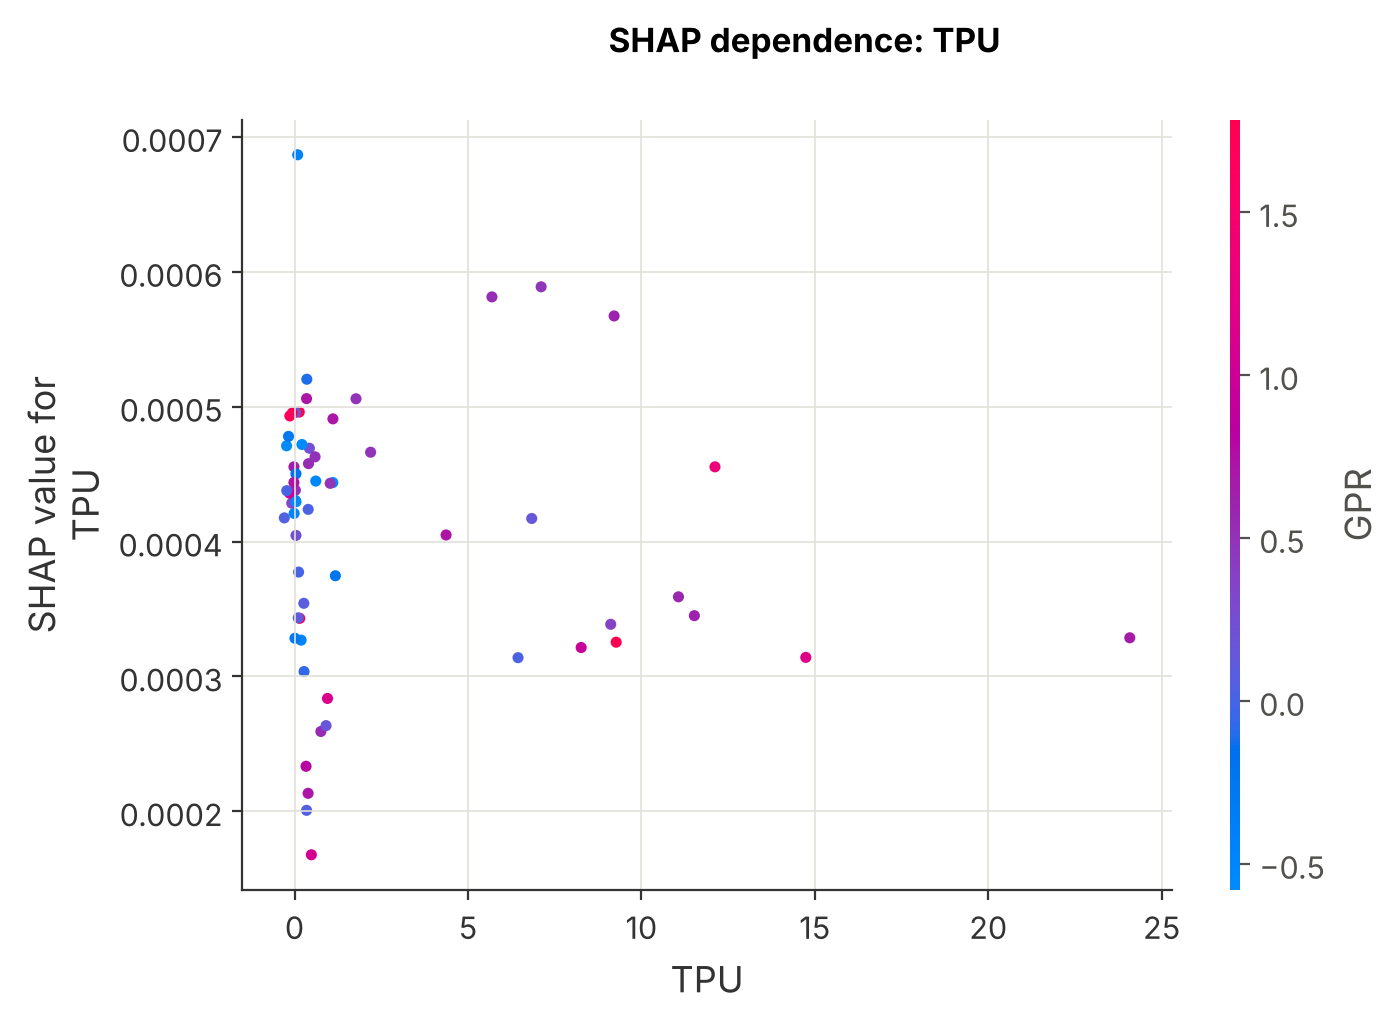
\includegraphics[width=\textwidth]{F15_shap_dependence_TPU.png}\caption{TPU (colour: GPR)}
  \end{subfigure}\hspace{0.05\textwidth}
  \begin{subfigure}{0.40\textwidth}\centering
    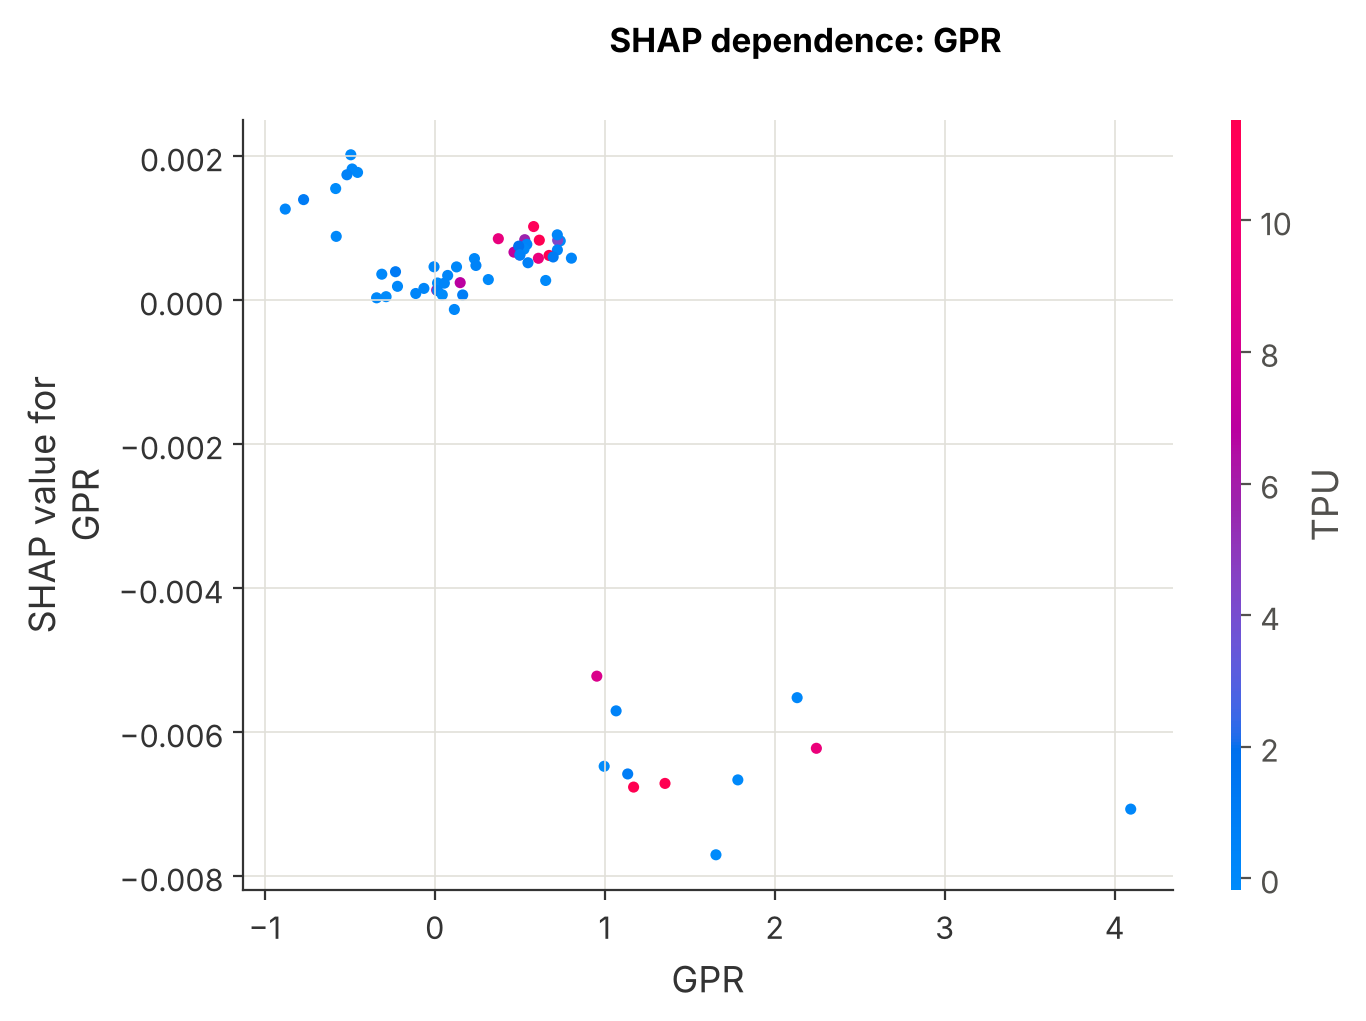
\includegraphics[width=\textwidth]{F15_shap_dependence_GPR.png}\caption{GPR (colour: TPU)}
  \end{subfigure}
  \caption{SHAP dependence plots for TPU and GPR (standardised feature values).}\label{fig:f15}
\end{figure*}

\figw{F16_ml_predictions.png}{0.92}{Out-of-sample predictions of each model against realised rolling volatility.}{fig:f16}
\figc{F17_ml_rmse_comparison.png}{1.0}{Out-of-sample RMSE by model; benchmarks highlighted.}{fig:f17}

% ================================================================== 7
\section{Discussion}\label{sec:discussion}

\subsection{The hypotheses}

Table~\ref{tab:hyp} summarises the evidence on the five hypotheses. The clearest result is negative: trade policy uncertainty does not raise Indian equity volatility in any of the models. The interaction of the two indices is never significant, so there is no evidence that trade and geopolitical uncertainty reinforce each other.

\begin{table*}[!t]\centering\small
\caption{Summary of the evidence}\label{tab:hyp}
\begin{tabularx}{\textwidth}{>{\raggedright\arraybackslash}p{3.6cm} >{\raggedright\arraybackslash}p{2.6cm} L}
\toprule
Hypothesis & Assessment & Evidence \\
\midrule
H1: TPU raises volatility & Not supported & GARCH-X variance coefficient negative and significant only at 10\%; insignificant in both ARDLs, the SVAR and every month of the TVP regression. \\
H2: GPR raises volatility & Rejected; effect negative & ARDL(1,0) long-run multiplier $-0.00125$ ($p=0.026$); negative TVP coefficient in 2020--22; negative SHAP contributions in months of high GPR. \\
H3: TPU and GPR reinforce each other & Not supported & Interaction insignificant at every lag and in every TVP month; negligible LASSO coefficient. \\
H4: Effects are stronger in crises & Partly supported & GFC dummy positive and significant; the only significant uncertainty effect in the TVP regression falls in the pandemic period; no crisis effect of TPU. \\
H5: US monetary policy uncertainty is transmitted to Indian volatility & Supported & Positive long-run MPU multiplier in both ARDLs ($p=0.023$ and $0.005$); MPU retained by the LASSO. \\
\bottomrule
\end{tabularx}
\end{table*}

The negative effect of geopolitical risk is the least expected result, and two interpretations are possible. Most large GPR episodes in the sample concern conflicts far from India, notably 2001--2003 and 2022. In such episodes international investors may treat India as a relatively insulated market, or domestic investors may reduce trading, either of which would dampen volatility. Alternatively, the result may be specific to the pandemic period, when geopolitical risk was low and volatility high; the time-varying estimates point in this direction. The sign is consistent across methods, but the magnitude is modest: a one-standard-deviation rise in GPR lowers long-run volatility by about 6\%.

\subsection{Persistence}

The most robust feature of the data is the persistence of volatility. The autoregressive coefficient is between 0.83 and 0.87 in both ARDL models, own shocks explain more than 99\% of the forecast-error variance in the SVAR, and the naive forecast achieves an out-of-sample $R^2$ of 0.79. The half-life of a shock is close to four months, so an episode of high volatility takes about a year to dissipate by 90\%. Uncertainty shocks may help trigger such episodes, but once an episode is under way they explain little of its evolution.

\subsection{Machine learning and econometrics}

The machine-learning results reinforce rather than challenge the econometric evidence. The best learners, the LASSO and the elastic net, reduce to an autoregression augmented with the VIX and MPU, and still fall slightly short of the AR(1). The tree ensembles fail because the test period lies at the edge of the training distribution, where trees cannot extrapolate. With about 250 training months and a single dominant autoregressive component, flexible models have little signal to exploit. Claims that machine learning improves volatility forecasts for India should therefore be evaluated against persistence benchmarks; in this sample they do not pass that test.

% ================================================================== 8
\section{Robustness}\label{sec:robust}

Table~\ref{tab:rob} summarises the robustness checks. The main conclusions are unchanged across specifications, orderings, smoothing parameters and data treatments.

\begin{table*}[!t]\centering\small
\caption{Robustness checks}\label{tab:rob}
\begin{tabularx}{\textwidth}{>{\raggedright\arraybackslash}p{3.8cm} L}
\toprule
Check & Result \\
\midrule
ARDL specification & The ARDL(2,2) in levels and the ARDL(1,0) in logs both reject the absence of a level relationship, both find TPU insignificant, and both give a negative long-run effect of the exchange rate and a positive effect of MPU. \\
Bounds test & In the error-correction form, the $t$-statistic on lagged volatility is $-5.33$ (base) and $-6.14$ (log specification); the $F$-statistic on the lagged regressor levels alone is 2.81 and 5.83. The level relationship in the log specification does not rest on the mean reversion of volatility alone. \\
Event dummies & Both dummies pass the screening in both specifications. The GFC dummy is significant (5\% in logs, 10\% in levels); the COVID-19 dummy is not. \\
Call money rate correction & With the uncorrected March 2007 value the GPR short-run coefficient in the log specification has $p=0.033$; with the corrected value $p=0.062$. Other results are unchanged. \\
Johansen lag length & Full rank in the three-variable system with zero, one or two lagged differences. \\
SVAR ordering & With GPR ordered before TPU, the peak TPU response changes from 0.187 to 0.186 points and its 24-month variance share from 0.91\% to 0.90\%. \\
TVP state variance & For $Q$ between 0.001 and 0.02, TPU is never significant; the negative GPR spell lasts between 8 and 31 months, always within 2020--22. The log-likelihood increases with $Q$ over this range, so $Q=0.005$ is a smoothing choice. \\
Output gap construction & Linking the IIP bases on a 12-month average ratio changes the gap by at most 0.52 percentage points (correlation 0.9998). \\
GARCH-X estimation & Ten random starting values reach the same optimum (log-likelihood $-1022.68$). \\
Parameter stability & CUSUM tests do not reject stability in either ARDL ($p=0.94$ and 0.72). \\
\bottomrule
\end{tabularx}
\end{table*}

% ================================================================== 9
\section{Conclusions}\label{sec:conclusion}

\subsection{Summary of findings}

This paper has examined whether global trade policy uncertainty and geopolitical risk affect the volatility of the Indian stock market, using monthly data from 1999 to 2025 and a sequence of complementary methods: a GARCH-X model of returns, ARDL bounds tests, a recursively identified structural VAR, a time-varying-parameter regression and a set of machine-learning models evaluated out of sample. The main findings can be stated briefly.

\begin{enumerate}
  \item Trade policy uncertainty does not raise Indian equity volatility. Its coefficient in the GARCH-X variance equation is small and negative and significant only at the 10\% level, and it is insignificant in both ARDL specifications, in the structural VAR and in every month of the time-varying regression, including the tariff escalation of 2025.
  \item Geopolitical risk is associated with slightly lower volatility. Its long-run multiplier in the log-volatility ARDL implies a fall of about 6\% in volatility per standard deviation of the index, but the effect is significant only at 5\% in the long run and 10\% in the short run, and it is concentrated in 2020--22.
  \item The two indices do not reinforce each other: their interaction is insignificant in every specification.
  \item Uncertainty about US monetary policy is the one uncertainty measure with a consistent positive effect on Indian volatility, in both ARDL models and in the variables retained by the LASSO.
  \item Volatility is dominated by its own dynamics. Own shocks account for more than 99\% of its forecast-error variance at every horizon up to two years, and the half-life of a shock is close to four months.
  \item No machine-learning model improves on an AR(1) forecast out of sample; the best penalised regressions are statistically indistinguishable from it and the tree ensembles are significantly worse.
\end{enumerate}

\subsection{Interpretation}

Taken together, the results do not support the view that headline trade-policy or geopolitical uncertainty is an important driver of volatility in Indian equities. This is a substantive finding rather than an inconclusive one. The absence of a TPU effect is consistent across five methods, across alternative specifications, orderings and smoothing parameters, and across periods, including the episode in which the index reached its historical maximum. Where uncertainty shocks of this kind matter for India, they appear to be absorbed in the level of prices, or to operate at frequencies too short to be visible in monthly volatility, rather than to raise the variability of returns over months.

The positive role of US monetary policy uncertainty points to the channel through which external shocks do reach Indian equities. Uncertainty about the path of US interest rates affects global risk appetite, portfolio flows to emerging markets and the rupee, and the evidence here suggests that these financial linkages matter more for Indian volatility than news about trade policy or international conflict. The positive long-run effect of the VIX is consistent with the same interpretation.

The negative effect of geopolitical risk admits two readings. Most large geopolitical episodes in the sample concern conflicts far from India, during which international investors may regard India as relatively insulated. Alternatively, the result may reflect a single period, the pandemic, in which geopolitical risk was low and volatility high. The time-varying estimates favour the second reading, and the result should be regarded as suggestive rather than established.

The persistence of volatility has a direct economic meaning. Periods of market stress, once begun, run their course over many months largely independently of subsequent movements in the uncertainty indices: with a half-life of about four months, an episode of high volatility takes roughly a year to dissipate by 90\%. This also explains the machine-learning results. When most of the predictable variation in volatility is captured by its own lag, flexible models have little additional signal to find, and with about 250 training months they are more likely to fit noise than structure.

\subsection{Policy implications}

Four implications follow. First, because volatility is highly persistent, monitoring that relies on current readings of uncertainty indices will understate how long market stress lasts; recent realised volatility is the most informative single indicator. Second, the role of US monetary policy uncertainty suggests that spillovers from Federal Reserve policy deserve more weight in Indian financial-stability assessment than trade-policy news, and that clear domestic monetary communication can help offset imported uncertainty. Third, global risk appears to reach Indian equities mainly through broad measures of risk aversion such as the VIX rather than through trade or geopolitical headlines. Fourth, acute global crises such as 2008--09 raise volatility beyond what these channels explain, which argues for crisis-specific rather than index-based contingency planning.

\subsection{Limitations}

Several limitations qualify these conclusions.

\begin{itemize}
  \item \textbf{Association rather than causation.} The structural VAR relies on a recursive ordering, and the ARDL and time-varying coefficients measure conditional associations. None of the estimates identifies the causal effect of an exogenous uncertainty shock.
  \item \textbf{The volatility measure.} Rolling twelve-month volatility is smooth and overlapping: consecutive observations share eleven months of returns. This inflates measured persistence, induces serial correlation in regression residuals and blurs short-lived shocks.
  \item \textbf{Frequency.} Monthly data may be too coarse to detect uncertainty effects that dissipate within days or weeks, so the null result for TPU applies to monthly volatility and should not be extended to daily market reactions.
  \item \textbf{Common trends.} The long-run relationship found in the bounds tests is driven largely by the exchange rate. Over the sample the rupee depreciated steadily while Indian equity volatility trended down, so part of this relationship reflects two trending series rather than a structural link.
  \item \textbf{Measurement of uncertainty.} The TPU index is built from US and UK newspapers and measures global rather than India-specific trade policy uncertainty. TPU and its interaction with GPR are also highly collinear (correlation 0.97), which limits the precision of their separate estimates.
  \item \textbf{The output gap.} The Hodrick--Prescott filter is two-sided and least reliable at the ends of the sample, so the output gap uses information not available in real time. The variable is insignificant throughout, so this does not affect the conclusions.
  \item \textbf{Sample size for machine learning.} With about 250 training observations and 61 test months, the comparison of forecasting models has limited power to detect small differences.
\end{itemize}

\subsection{Directions for further research}

The most useful extension would re-estimate the core models with realised volatility from daily NIFTY returns or with the India VIX, which would remove the overlap in the rolling measure and allow short-lived shocks to be identified. An India-specific uncertainty measure, such as the Indian Economic Policy Uncertainty index of \citet{baker2016}, or a decomposition of trade policy uncertainty into threats and implemented measures, would sharpen the question. Event studies around specific tariff announcements and local projections conditioned on the state of the market would provide more credible identification. Finally, a joint model of volatility, portfolio flows and the exchange rate would allow a direct test of the safe-haven interpretation of the geopolitical-risk result and of the monetary-spillover channel.

% ================================================================== references
\renewcommand{\bibfont}{\small\raggedright}
\bibliographystyle{apalike}
\bibliography{references}

% ================================================================== appendix
\appendix
\section{Additional figures}

\figc{FA2_output_gap_zoom.png}{1.0}{Output gap on a truncated scale; the April 2020 observation ($-82.7\%$) lies off the scale.}{fig:fa2}

\section{Data availability and replication}

The analysis can be reproduced from the accompanying code repository, which contains the estimation code, all results tables and figures, and the series that are publicly available: the NIFTY~50 prices, the TPU and GPR indices, the US monetary and economic policy uncertainty indices and the VIX. The Indian macroeconomic series (the Index of Industrial Production on the 1993-94, 2004-05 and 2011-12 bases, consumer price inflation, the rupee--dollar exchange rate and the call money rate) were obtained from CEIC, a subscription database whose terms do not permit redistribution. They are therefore not included in the public repository. The repository documents the CEIC series used, including the identifiers of the three IIP series (18989701, 314398401 and 386587797), so that users with CEIC access can download them and place them in the folders indicated to reproduce every result.

\medskip
\noindent\textbf{Code repository:} % TODO: replace with the final repository URL
\url{https://github.com/himdev20/TPU_GPR_Market_volatility}

\end{document}
